%%%%%%%%%%%%%%%%%%%%%%%%%%%%%%%%%%%%%%%%%
% Short Sectioned Assignment LaTeX Template Version 1.0 (5/5/12)
% This template has been downloaded from: http://www.LaTeXTemplates.com
% Original author:  Frits Wenneker (http://www.howtotex.com)
% License: CC BY-NC-SA 3.0 (http://creativecommons.org/licenses/by-nc-sa/3.0/)
%%%%%%%%%%%%%%%%%%%%%%%%%%%%%%%%%%%%%%%%%

%----------------------------------------------------------------------------------------
%	PACKAGES AND OTHER DOCUMENT CONFIGURATIONS
%----------------------------------------------------------------------------------------

\documentclass[paper=a4, fontsize=11pt]{scrartcl} % A4 paper and 11pt font size

% ---- Entrada y salida de texto -----

\usepackage[T1]{fontenc} % Use 8-bit encoding that has 256 glyphs
\usepackage[utf8]{inputenc}
%\usepackage{fourier} % Use the Adobe Utopia font for the document - comment this line to return to the LaTeX default

% ---- Idioma --------

\usepackage[spanish, es-tabla]{babel} % Selecciona el español para palabras introducidas automáticamente, p.ej. "septiembre" en la fecha y especifica que se use la palabra Tabla en vez de Cuadro

% ---- Otros paquetes ----

% Hipervínculos
\usepackage[hidelinks]{hyperref}

\usepackage{amsmath,amsfonts,amsthm} % Math packages
%\usepackage{graphics,graphicx, floatrow} %para incluir imágenes y notas en las imágenes
\usepackage{graphics,graphicx, float, url} %para incluir imágenes y colocarlas

% Para hacer tablas comlejas
%\usepackage{multirow}
%\usepackage{threeparttable}

%\usepackage{sectsty} % Allows customizing section commands
%\allsectionsfont{\centering \normalfont\scshape} % Make all sections centered, the default font and small caps

\usepackage{fancyhdr} % Custom headers and footers
\pagestyle{fancyplain} % Makes all pages in the document conform to the custom headers and footers
\fancyhead{} % No page header - if you want one, create it in the same way as the footers below
\fancyfoot[L]{} % Empty left footer
\fancyfoot[C]{} % Empty center footer
\fancyfoot[R]{\thepage} % Page numbering for right footer
\renewcommand{\headrulewidth}{0pt} % Remove header underlines
\renewcommand{\footrulewidth}{0pt} % Remove footer underlines
\setlength{\headheight}{13.6pt} % Customize the height of the header

\numberwithin{equation}{section} % Number equations within sections (i.e. 1.1, 1.2, 2.1, 2.2 instead of 1, 2, 3, 4)
\numberwithin{figure}{section} % Number figures within sections (i.e. 1.1, 1.2, 2.1, 2.2 instead of 1, 2, 3, 4)
\numberwithin{table}{section} % Number tables within sections (i.e. 1.1, 1.2, 2.1, 2.2 instead of 1, 2, 3, 4)

\setlength\parindent{0pt} % Removes all indentation from paragraphs - comment this line for an assignment with lots of text

\newcommand{\horrule}[1]{\rule{\linewidth}{#1}} % Create horizontal rule command with 1 argument of height

%----------------------------------------------------------------------------------------
%	TÍTULO Y DATOS DEL ALUMNO
%----------------------------------------------------------------------------------------

\title{	
\normalfont \normalsize 
\textsc{{\bf Ingeniería de Servidores (2015-2016)} \\ Doble Grado en Ingeniería Informática y Matemáticas \\ Universidad de Granada} \\ [25pt] % Your university, school and/or department name(s)
\horrule{0.5pt} \\[0.4cm] % Thin top horizontal rule
\huge Memoria Práctica 1 \\ % The assignment title
\horrule{2pt} \\[0.5cm] % Thick bottom horizontal rule
}

\author{Óscar Bermúdez Garrido\\ \href{http://www.github.com/oxcar103}{@oxcar103}} % Nombre y apellidos

\date{\normalsize\today} % Incluye la fecha actual

%----------------------------------------------------------------------------------------
% DOCUMENTO
%----------------------------------------------------------------------------------------

\begin{document}

\maketitle % Muestra el Título

\newpage %inserta un salto de página

\tableofcontents % para generar el índice de contenidos

\listoffigures

\listoftables

\newpage


\begin{enumerate}
	\section{Introducción}
	\subsection{Concepto de Máquina Virtual y virtualización}
		\item ¿Qué modos y/o tipos de $"$Virtualización Hardware$"$ existen?
		\begin{itemize}
			\item Emulación: La máquina virtual \textit{emula} el hardware, a partir del existente
			en la máquina, para ejecutar un sistema operativo que normalmente estaba pensado para
			otro tipo de dispositivo.
			
			\item Virtualización completa o nativa: La máquina virtual simula parte del hardware de
			la máquina para ejecutar un sistema operativo \textit{invitado} de forma autónoma.
			
			\item Para-virtualización: Es similar a la virtualización nativa pero con la diferencia
			de que el sistema \textit{invitado} que se ejecuta está modificado para enviar ciertas
			peticiones al sistema \textit{anfitrión} que si se ejecutaran en el entorno virtualizado
			serían mucho menos eficientes.
		\end{itemize}
		\cite{Virt}
		
		\item Muestre los precios y características de varios proveedores de VPS(Virtual Private
		Server) y compare con el precio de servidores dedicados(administrados y no administrados)
		de características similares. Comente diferencias.
		
		En Softlayer\cite{VPS_IBM}, podemos configurar más a la medida las características de
		nuestro servidor que en otros sitios webs ya que podemos seleccionar el número de CPU's,
		cantidad de RAM, número y memoria de los discos duros, sistema operativo,... por separado
		en lugar de tomar una oferta u otra del resto de páginas como Gigas\cite{VPS_Gigas} y
		Axarnet, éste último nos ofrece VPS no administrados\cite{VPS_Axarnet} y administrados con
		panel Plesk 12\cite{VPS_Axarnet_admin} o cPanel\cite{VPS_Axarnet_admin_2}.
		
		Un servidor linux con 2GB de ram, 2 núcleos y 25GB de disco(aprox.), cuesta $53.40\$$
		\cite{VPS_IBM}, $17.64\$$\cite{VPS_Gigas}, $10.7\$$\cite{VPS_Axarnet} ó $16.06\$$
		\cite{VPS_Axarnet_admin} dependiendo de dónde se contrate.
		
		Un servidor linux con 4GB de ram, 4 núcleos y 50GB de disco(aprox.), cuesta $113.96\$$
		\cite{VPS_IBM}, $32.38\$$\cite{VPS_Gigas}, $16.06\$$\cite{VPS_Axarnet}, $21.42\$$
		\cite{VPS_Axarnet_admin} ó $35.69\$$\cite{VPS_Axarnet_admin_2} dependiendo de dónde se contrate.
		
		Un servidor linux con 8GB de ram, 8 núcleos y 100GB de disco(aprox.), cuesta $220\$$
		\cite{VPS_IBM}, $77.06\$$\cite{VPS_Gigas}, $26.78\$$\cite{VPS_Axarnet}, $32.14\$$
		\cite{VPS_Axarnet_admin} ó $53.56\$$\cite{VPS_Axarnet_admin_2} dependiendo de dónde se contrate.
		
		Es reseñable el hecho de que los precios mensuales varían dependiendo del sistema operativo
		que optemos por instalar. Pues si instalamos un servidor de Windows en \cite{VPS_IBM} nos
		costará $17\$$ y unos $20\$$ en \cite{VPS_Axarnet} y \cite{VPS_Axarnet_admin}; y en
		\cite{VPS_IBM}, si optamos por coger Red Hat Enterprise Linux nos costará $45\$$. También es
		considerable la diferencia de precios para un mismo servicio entre estar administrado y no
		estarlo (\cite{VPS_Axarnet} y \cite{VPS_Axarnet_admin}).
		
		\item ¿Qué otros software de virtualización existen además de VMWare y Virtual Box?
		Como podemos ver en \cite{VMSW}, existe una amplia variedad de alternativas a la hora de
		escoger máquina virtual, de las cuáles destacaré:
		
		\begin{itemize}
			\item Adaptive Domain Environment Operating Systems(\textbf{ADEOS}\cite{Adeos}) permite
			la ejecución de múltiples instancias de sistemas operativos principalmente mediante
			virtualización nativa.
			
			\item \textbf{QEMU}\cite{QEMU} es un emulador de procesadores sin interfaz gráfica por
			defecto (por lo que tiene un soporte incompleto de controladores multimedia para los
			sistemas \textit{invitado}).
			
			\item \textbf{DOSEMU}\cite{DOSEMU} y \textbf{DOSBox}\cite{DOSBox} permiten emular al
			sistema operativo DOS con la diferencia de que el primero está especialmente diseñado
			para Linux y el segundo es multiplataforma.
			
			\item Kernel-based Virtual Machine(\textbf{KVM}\cite{KVM}) que es una estructura de 
			virtualización integrada directamente en el \textit{kernel} de Linux desde 2007 y que
			permite virtualización nativa de otros SO's.
		\end{itemize}
		
		Todas las aplicaciones listadas en este apartado se distribuyen bajo la licencia
		\href{https://www.gnu.org/licenses/gpl.html}{\textbf{GPL}}.
		
	\section{Instalación de Sistemas Operativos virtualizados}
		\item Enumere algunas de las innovaciones en Windows 2012 R2 respecto a 2008R2.
		
		Windows 2012 destaca principalmente por:
		\begin{itemize}
			\item \textbf{Servicios de Cloud}\cite{Hoja_Datos}\cite{Overview}\cite{TechWeek}:
			Está basado en Hyper-V para la configuración y despliegue de servicios cloud, como
			puede ser la utilización de servicios desde cualquier dispositivo y lugar. Además,
			permite agilizar los procesos de gestión y administración, así como da mayor
			protección de la información.
			
			\item \textbf{Almacenamiento}\cite{TechWeek}: Tiene un nuevo sistema de gestión de
			ficheros que tiene mayor fiabilidad y recuperación en estructuras de disco, además
			de compatibilidad con las tecnologías existentes.
			
			\item \textbf{Administración}\cite{TechWeek}: Implementa más de 2000 comandos
			Powershell frente a los 200 de Windows Server 2008, además de una nueva interfaz
			que facilitará el proceso de administración.
			
			\item \textbf{Orientado a las aplicaciones}\cite{Hoja_Datos}\cite{Overview}: Ayuda a
			desarrollar y escalar aplicaciones con mayor rapidez y flexibilidad. Permite mayor
			soporte para los estándares abiertos, así como para aplicaciones de código abierto y
			varios lenguajes de desarrollo de aplicaciones.
			
			\item \textbf{Centrado en el usuario}\cite{Hoja_Datos}\cite{Overview}:Permite acceso
			más rápido y flexible. Además, se protege mejor la información crítica y ayuda a
			evitar riesgos validando definiendo niveles de acceso que los usuarios tienen en
			función de quiénes son, a lo que quieren acceder o la infraestructura que están usando.
		\end{itemize}
		
		\item ¿Qué empresa hay detrás de Ubuntu?¿Qué otros productos/servicios ofrece?
		
		El sistema operativo Ubuntu\cite{Ubuntu} es desarrollado por la comunidad de Ubuntu y por la
		empresa británica Canonical Ltd.\cite{Canonical}.
		
		Esta empresa también desarrollada otros proyectos de software libre. Entre ellos:
		
		\begin{itemize}
			\item \textit{Mir}: Servidor gráfico que se planea que sea el sustituto de \textit{X
			Windows Server} para Ubuntu.
			
			\item \textit{Bazaar}: Sistema de control de versiones(especialmente para python).
			
			\item \textit{Juju}: Herramienta de organización de servicios.
			
			\item \textit{MAAS}\cite{MAAS} que permite el acceso y administración de un conjunto de
			servidores(principalmente desarrollado para Ubuntu Server) de forma similar a como se
			utilizarían los servicios de cloud utilizando \textit{Juju}.
		\end{itemize}
		
		De nuevo, bajo la licencia \href{https://www.gnu.org/licenses/gpl.html}{\textbf{GPL}}.
		
		\item ¿Qué relación tiene CentOS con RedHat y con el proyecto Fedora?
		
		Tanto Fedora\cite{Fedora}, como CentOS\cite{CentOS}, como Red Hat Enterprise Linux\cite{RedHat}
		son marcas que pertenecen a RedHat Inc.
		
		Originalmente, la empresa tenía una distribución comercial llamada Red Hat Linux que fue
		abandonada por la nueva distribución (RHEL), basándose en ella, apareció Fedora como proyecto
		comunitario con una gran comunidad de ingenieros, entre ellos \textit{Linus Torvalds}. Fedora
		se caracteriza por tener como objetivo la innovación e integración de nuevas tecnologías. De
		hecho, se dice que hablar del progreso de Fedora es hablar del progreso del software libre
		y el código abierto\cite{cita}.
		
		Por su parte, RHEL quedó como la distribución oficial, se basa en Fedora para su desarrollo
		pero con soporte técnico por la empresa, para lo cuál es necesario el abono de un importe.
		
		Más tarde, apareció CentOS como una distribución formada a partir del código que libera
		RHEL debido a su licencia. Por lo que está soportada, de forma indirecta, por RedHat Inc.
		aunque de forma directa por su propia comunidad de desarrolladores.
		
		También tienen en común la licencia \href{https://www.gnu.org/licenses/gpl.html}{\textbf{GPL}}.
		
		\item Indique qué otros SO se utilizan en servidores y el porcentaje de uso(no olvide poner
		la fuente de donde saca la información y preste atención a la fecha de esta).
		
		De los servidores web cuyo sistema operativo es conocido con fecha del 25 de marzo de 2016:
		\newline El $68,0\%$ usan Unix, el $32,0\%$ usa Windows y menos del $0,1\%$ utiliza OS X
		\cite{Market_Share_global} (proporción que se ha mantenido desde el 2010 con un margen del 5\%).
		\cite{Market_Share_yearly}
		
		Además, de entre los que utilizan Unix, el $53,3\%$ usa Linux, el $1,3\%$ usa BSD menos del
		$0,1\%$ usan Darwin, HP-UX o Solaris y el $45,4\%$ es desconocido.\cite{Market_Share_unix}
		
		Más específicamente, de entre los que utilizan linux, el $32,5\%$ usa Debian, el $31,4\%$
		usan Ubuntu, el $20,3\%$ usa CentOS, el $3,9\%$ utilizan Red Hat, el $2,7\%$ optan por Gentoo,
		el $1,1\%$ prefiere Fedora, el $1,0\%$ elige SuSE, una lista de 8 distribuciones a menos de
		$0,1\%$ cada una y el $6,8\%$ es desconocido.\cite{Market_Share_linux}
		
	\subsection{Linux: Particionamiento del Disco Duro virtual y creación de RAID1}
		\item ¿Qué diferencia hay entre RAID mediante SW y mediante HW?\\
		Un RAID mediante hardware es un controlador(normalmente, en forma de tarjeta) que permite gestionar
		el sistema de forma independiente y dando la sensación a la máquina de que hay un único disco mientras
		que en el RAID por software es el propio software el encargado de tratar los discos como un RAID.
		
		Mientras que el RAID por software es más barato(ya que es parte del sistema operativo) y es mejor
		para RAID 0 ó RAID 1, el RAID por hardware es más simple y permite \textit{$"$hot swap$"$}.
		\cite{HWvsSW}\cite{RAID_RedHat}
		
		
		\item \begin{enumerate}
			\item ¿Qué es LVM?
			
			LVM es un administrador de volúmenes lógicos para el kernel Linux que administra
			controladores de discos y dispositivos de almacenamiento masivo similares.\cite{LVM}
			
			\item ¿Qué ventaja tiene para un servidor de gama baja?
			
			Permite la gestión de los discos disponibles y sus particiones de una forma lógica de
			tal forma que si próximamente una parte se queda sin espacio, podemos fácilmente
			redimensionarla y tomar espacio de otra a la que le sobre o incorporar un nuevo disco
			sin necesidad de copiar los datos que necesita guardar, simplemente, lo repartimos
			entre las particiones disponibles. Esto nos permite realizar \textit{$"$hot swap$"$}
			de los discos que disponemos si fuese necesario.
			
			\item Si va a tener un servidor web, ¿le daría un tamaño grande o pequeño a /var?\\
			(\href{http://www.tldp.org/HOWTO/LVM-HOWTO/benefitsoflvmsmall.html}
			{http://www.tldp.org/HOWTO/LVM-HOWTO/benefitsoflvmsmall.html})\\
			(\href{https://wiki.archlinux.org/index.php/LVM#Introduction}
			{https://wiki.archlinux.org/index.php/LVM$\#$Introduction})
			
			Dado que el directorio /var es un directorio multipropósito en el cuál se almacenan
			todos los archivos temporales, log, \dots que necesite usar el sistema operativo\cite{Var}
			el tamaño que necesitará si pretendemos alojar un servidor web dependerá de las prestaciones
			que aportemos con dicho servidor, usualmente grande. Como no sabemos a priori si el espacio
			que le hemos dado será suficiente y es posible que necesitemos ampliarlo, si disponemos de
			LVM, podemos optar por darle poco espacio inicialmente e irlo redimensionando conforme se
			requiera más espacio.
			
		\end{enumerate}
		
		\item ¿Debemos cifrar también el volumen que contiene el espacio para swap? ¿y el volumen
		en el que montaremos /boot?
		
		Dado que el espacio para swap puede llegar a contener información crítica, tanto del sistema como
		de los usuarios(claves de acceso, datos personales,...), se recomienda cifrarla o, si se puede 
		prescindir de ella, omitir dicha partición\cite{swap}. Sin embargo, /boot no se puede cifrar porque
		es necesaria la encriptación de la carpeta /root\cite{boot}, además, dado que el contenido de dicha
		carpeta es propio del sistema operativo e idéntico entre sistemas operativos iguales, no tendría mucho
		sentido.
		
		\item ¿Qué otro tipo de usos de una partición le permite configurar el asistente de instalación?
		¿Cuál es la principal diferencia entre ext4 y ext2?
		
		El asistente de configuración nos permite seleccionar entre \textbf{ext2}\cite{ext2},
		\textbf{ext3}\cite{ext3}, \textbf{ext4}\cite{ext4} que suelen ser los sistemas de ficheros más
		usados; \textbf{btrfs}\cite{btrfs} que se desarrolló como una alternativa a ellos de manos de
		uno de sus desarrolladores, \textit{Theodore Ts'o}, buscando solventar algunas de las
		deficiencias de los mismos; \textbf{JFS}\cite{JFS} y \textbf{XFS}\cite{XFS} que están más
		enfocados a las altas prestaciones así como a archivos de mayor tamaño que a uso habitual
		aunque también dan buenos resultados; y sistemas de ficheros \textbf{FAT}\cite{FAT} que,
		junto con \textbf{NTFS}\cite{NTFS}, son más característicos de los sistemas basados en
		\textbf{DOS}.
		
		Ahora bien, centándonos en \textbf{ext2}, \textbf{ext3} y \textbf{ext4}, tenemos que como son
		mejoras entre ellos, las versiones nuevas tienen las mismas características que sus predecesores
		e incorporan ciertas soluciones a los problemas que tenían.
		\newline
		En concreto, \textbf{ext3} mejora a \textbf{ext2} mediante la indexación (usando árboles
		\textit{HTree}) de grandes directorios, el crecimiento lineal del sistema de archivos y, la
		gran diferencia, el \textit{journaling}\cite{journaling}, que consiste en ir guardando las
		diferencias producidas a diario y así, en caso de un fallo o reinicio inesperado, se permite
		una recuperación más eficiente del estado del sistema antes de producirse dicho error.
		\newline
		Por su parte, \textbf{ext4} mejora a \textbf{ext3} principalmente por la ampliación del tamaño
		máximo de sus ficheros, el del sistema de archivos en sí y el número máximo de subdirectorios.
		
		Aún así, quedan algo alejados de los límites máximos de \textbf{JFS} y \textbf{XFS}.
		
		\item Muestre cómo ha quedado el disco particionado una vez el sistema está instalado(lsblk).
		
		El disco ha quedado como muestra la imagen siguiente:
		
		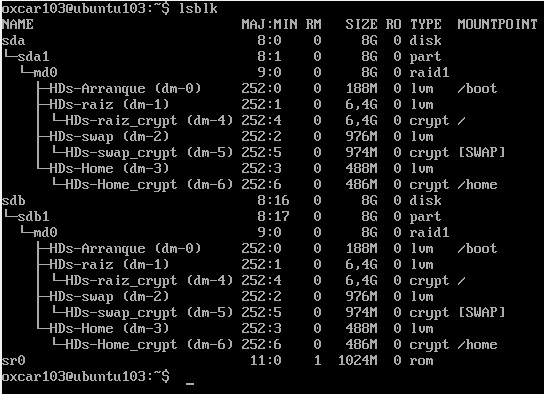
\includegraphics{Ejercicio_12.jpg}
		
		\item \begin{enumerate}
			\item ¿Cómo ha hecho el disco 2 $"$arrancable$"$?
			
			Para hacer disco 2 $"$arrancable$"$, localizamos el disco(usando el comando anterior,
			\textit{lsblk}, por ejemplo), ejecutamos \textit{grub install $<$dirección del dispositivo$>$}
			y finalmente, ejecutamos \textit{update-grub} para generar el archivo de menu.lst de GRUB.
			La salida por pantalla sería:
			
			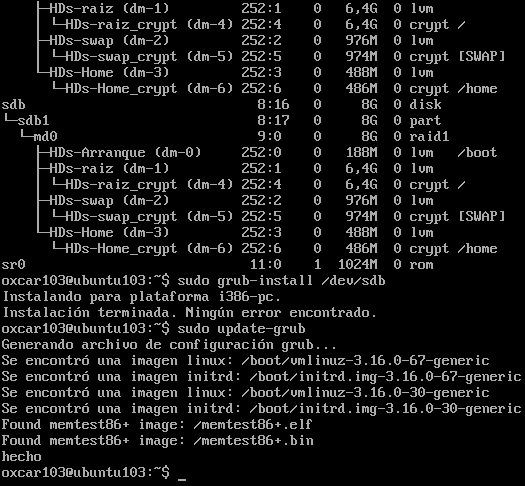
\includegraphics[width=15cm]{Ejercicio_13.jpg}
			
			\item ¿Qué hace el comando grub-install?
			
			El comando \textit{grub-install} instala un \textbf{GRUB} (\textit{GNU GRand Unified
			Bootloader}) en el dispositivo que se le pasa como parámetro con las opciones indicadas
			\cite{man_grub-install}.
			
			\item ¿Qué hace el comando dd?
			
			El comando \textit{dd} copia y convierte archivos archivos a bajo nivel, permitiendo configurar
			mediante los comandos adecuados la cantidad de bytes que se leen o escriben a la vez\cite{man_dd}.
			
		\end{enumerate}
		
		\item \textbf{Opcional:} Muestre(con capturas de pantalla) cómo ha comprobado que el RAID1
		funciona.
		
		
		
	\subsection{Windows Server}
		\item ¿Qué diferencia hay entre Standard y Datacenter?
		
		La principal diferencia entre ambas versiones es el número de máquinas virtuales que se
		permiten ejecutar. En la Standard se permite un máximo de 2 y en la Datacenter no hay
		límite.\cite{W12_v}
		
		\item Continúe usted con el proceso de definición de RAID1 para los 2 discos de 50MiB que
		ha creado. Muestre el proceso con capturas de pantalla.
		
		Mostraré dos métodos para realizar este proceso: 
		
		\textbf{Primer caso: teníamos un disco funcionando sin RAID1 y queremos incorporar un nuevo
		disco para comenzar a trabajar como RAID1}
		
		En este caso, pulsamos botón derecho sobre el volumen que tenemos y seleccionamos
		\textit{$"$Add Mirror...$"$} como podemos ver en la figura:
		
		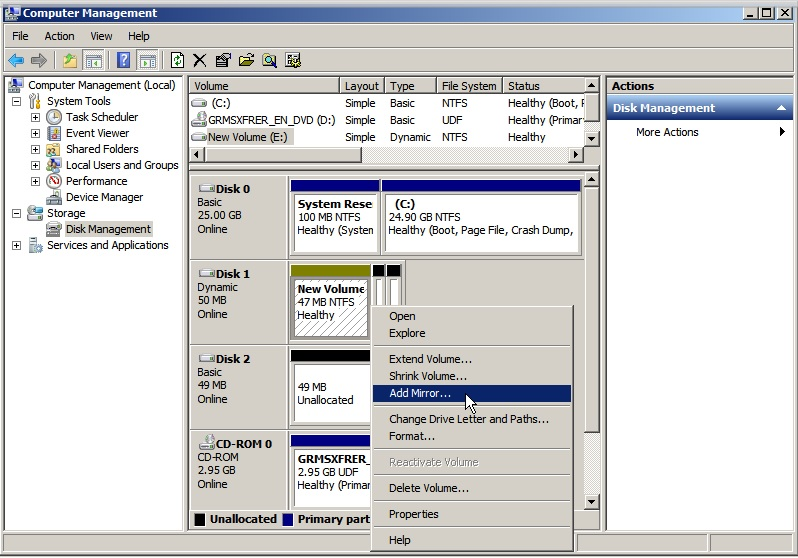
\includegraphics[width=10cm]{Ejercicio_16a.jpg}
		
		Seleccionamos el disco que queremos añadir como espejo:
		
		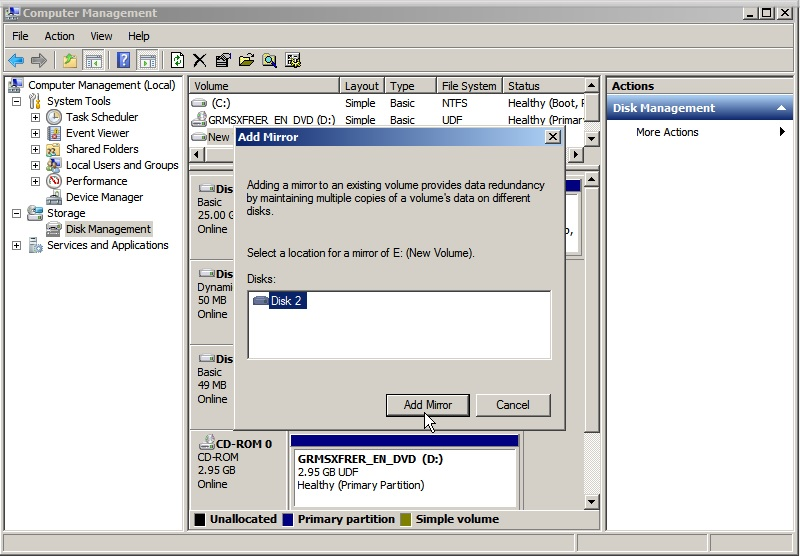
\includegraphics[width=10cm]{Ejercicio_16b.jpg}
		
		Y el resultado es:
		
		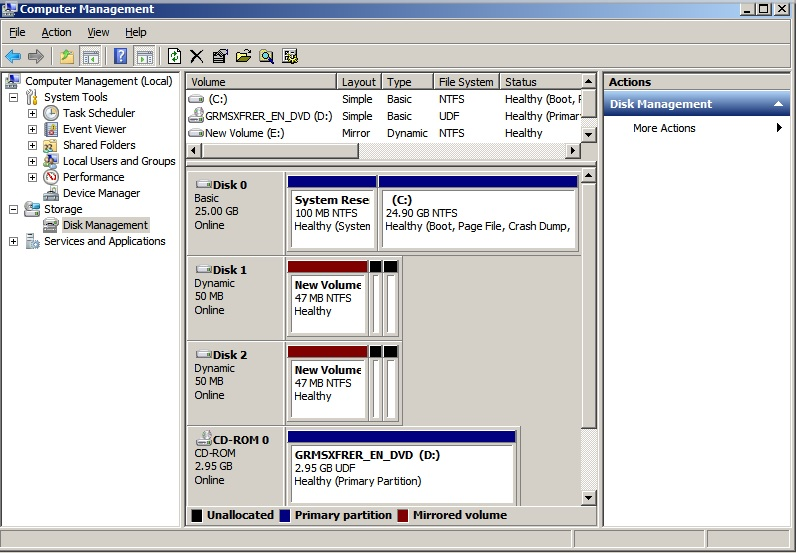
\includegraphics[width=10cm]{Ejercicio_16c.jpg}
		
		\textbf{Segundo caso: tenemos desde el principio los discos que queremos convertir en RAID1}
		
		
	\subsection{Ajuste de parámetros de la Máquina Virtual}
		\item Explique brevemente qué diferencias hay entre los 3 tipos de conexión que permite el
		VMSW para las Mvs: NAT, Red NAT, Bridge, Red interna y Host-only.
		\begin{itemize}
			\item NAT es equivalente a hacer una red virtual donde sólo se puede conectar una máquina
			virtual.
			\item Red NAT: nuestro sistema operativo va a hacer de anfitrión a tantos SO's como
			queramos, es equivalente a (el sistema operativo simula una capa de red).
			\item Bridge(adaptador puente): va a "puentear" la pila de red, se hace un filtrado de
			tráfico de red a transporte, útil para saber qué máquinas hablan con cuáles y similares.
			Capaz de tener más de una máquina a la vez.
			\item Red interna: va a "puentear" la pila de red, la diferencia es que el sistema operativo
			Host y los Guest no se ven.
			\item Host-only: lo mismo que la anterior pero se pueden ver.
		\end{itemize}
		
	\section{Editores de texto}
		\item \textbf{Opcional:} ¿Qué relación hay entre los atajos de teclado de emacs y los de
		la consola de bash?¿y entre los de vi y las páginas del manual?
		Son similares en avance de página y otras funciones de lectura. Por qué la similitud? Las
		funciones estaban implementadas en emacs y lo cogieron.
		
		
\end{enumerate}


\newpage
\section{Referencias}
\begin{thebibliography}{10}
\expandafter\ifx\csname url\endcsname\relax
  \def\url#1{\texttt{#1}}\fi
\expandafter\ifx\csname urlprefix\endcsname\relax\def\urlprefix{URL }\fi
\expandafter\ifx\csname href\endcsname\relax
  \def\href#1#2{#2} \def\path#1{#1}\fi

\bibitem{Virt}
LASS (Laboratory fo Advanced Software Systems)
  \url{http://lass.cs.umass.edu/~shenoy/courses/spring11/lectures/Lec05.pdf}

\bibitem{VMSW}
Virtual Machine. Wikipedia, the free encyclopedia.\\
  \url{https://en.wikipedia.org/wiki/Virtual_machine}

\bibitem{VPS_IBM}
Softlayer, an IBM Company.\\
  \url{http://www.softlayer.com/info/vps}\\
  \url{https://www.softlayer.com/Store/orderComputingInstance/1640,1644,2202}

\bibitem{VPS_Gigas}
Gigas, the cloud hosting company.\\
  \url{https://gigas.com/cloud-vps}

\bibitem{VPS_Axarnet}
Axarnet, VPS no administrado.\\
  \url{https://www.axarnet.es/servidores-vps/servidor-virtual-privado-no-administrado/}

\bibitem{VPS_Axarnet_admin}
Axarnet, VPS administrados.\\
  \url{https://www.axarnet.es/servidores-vps/windows-linux-server-administrado/}

\bibitem{VPS_Axarnet_admin_2}
Axarnet, VPS administrados(sólo linux).\\
  \url{https://www.axarnet.es/servidores-vps/linux-server-administrado/}

\bibitem{Adeos}
Adaptive Domain Environment for perating Systems. Wikipedia, the free encyclopedia.\\
  \url{http://en.wikipedia.org/wiki/Adaptive_Domain_Environment_for_Operating_Systems}

\bibitem{QEMU}
QEMU. Wikipedia, the free encyclopedia.\\
  \url{http://en.wikipedia.org/wiki/QEMU}

\bibitem{DOSEMU}
DOSEMU. Wikipedia, the free encyclopedia.\\
  \url{http://en.wikipedia.org/wiki/DOSEMU}

\bibitem{DOSBox}
DOSBox. Wikipedia, the free encyclopedia.\\
  \url{http://en.wikipedia.org/wiki/DOSBox}

\bibitem{KVM}
Kernel-based Virtual Machine. Wikipedia, the free encyclopedia.\\
  \url{http://en.wikipedia.org/wiki/Kernel-based_Virtual_Machine}

\bibitem{Hoja_Datos}
Windows Server 2012 R2 Datasheet, June 14, proporcionado por
\href{http://www.microsoft.com/es-es/server-cloud/products/windows-server-2012-r2/}{esta página}

\bibitem{Overview}
Windows Server 2012 R2 Overview, proporcionado por
\href{http://www.microsoft.com/es-es/server-cloud/products/windows-server-2012-r2/}{esta página}

\bibitem{TechWeek}
TechWeek, revista bisemanal de tecnología.\\
  \url{http://www.techweek.es/servidores/noticias/1011002005001/windows-server-2012-funciones-cloud-privado-publico-hyper-v.1.html}

\bibitem{Ubuntu}
Ubuntu. Wikipedia, the free encyclopedia.\\
  \url{http://en.wikipedia.org/wiki/Ubuntu_(operating_system)}

\bibitem{Canonical}
Canonical. Wikipedia, the free encyclopedia.\\
  \url{http://en.wikipedia.org/wiki/Canonical_(company)}

\bibitem{MAAS}
MAAS, Metal As A Service, the official website.\\
  \url{http://maas.ubuntu.com/docs1.5/}

\bibitem{Fedora}
Fedora. Wikipedia, the free encyclopedia.\\
  \url{http://en.wikipedia.org/wiki/Fedora_(operating_system)}

\bibitem{CentOS}
CentOS. Wikipedia, the free encyclopedia.\\
  \url{http://en.wikipedia.org/wiki/CentOS}

\bibitem{RedHat}
Red Hat Enterprise Linux. Wikipedia, the free encyclopedia.\\
  \url{http://en.wikipedia.org/wiki/Red_Hat_Enterprise_Linux}

\bibitem{cita}
Max Spevack, diciembre, 2006.\\
  Fedora Project Leader Max Spevack Responds\\

\bibitem{Market_Share_global}
W3Techs, Web Technology Surveys.\\
  \url{http://w3techs.com/technologies/overview/operating_system/all}

\bibitem{Market_Share_yearly}
W3Techs, Web Technology Surveys.\\
  \url{http://w3techs.com/technologies/history_overview/operating_system/ms/y}

\bibitem{Market_Share_unix}
W3Techs, Web Technology Surveys.\\
  \url{http://w3techs.com/technologies/details/os-unix/all/all}

\bibitem{Market_Share_linux}
W3Techs, Web Technology Surveys.\\
  \url{http://w3techs.com/technologies/details/os-linux/all/all}

\bibitem{HWvsSW}
Hardware RAID vs. Software RAID: Which Implementation is Best for my Application?\\
  \url{http://www.adaptec.com/nr/rdonlyres/14b2fd84-f7a0-4ac5-a07a-214123ea3dd6/0/4423_sw_hwraid_10.pdf}

\bibitem{RAID_RedHat}
Red Hat Enterprise Linux 3: Manual de administración del sistema.\\
  Capítulo 3. 3.3. Hardware y Software RAID.\\
  \url{http://web.mit.edu/rhel-doc/3/rhel-sag-es-3/s1-raid-approaches.html}

\bibitem{LVM}
Logical Volume Manager. Wikipedia, the free encyclopedia.\\
  \url{http://en.wikipedia.org/wiki/Logical_Volume_Manager_(Linux)}

\bibitem{Var}
The Linux Documentation Project.\\
  \url{http://www.tldp.org/LDP/Linux-Filesystem-Hierarchy/html/var.html}

\bibitem{swap}
Disk Encryption. Archlinux Wiki.\\
  \url{https://wiki.archlinux.org/index.php/Disk_encryption}

\bibitem{boot}
Encrypting an entire system. Archlinux Wiki.\\
  \url{https://wiki.archlinux.org/index.php/Dm-crypt/Encrypting_an_entire_system}

\bibitem{ext2}
Ext2. Wikipedia, the free encyclopedia.\\
  \url{http://en.wikipedia.org/wiki/Ext2}

\bibitem{ext3}
Ext3. Wikipedia, the free encyclopedia.\\
  \url{http://en.wikipedia.org/wiki/Ext3}

\bibitem{ext4}
Ext4. Wikipedia, the free encyclopedia.\\
  \url{http://en.wikipedia.org/wiki/Ext4}

\bibitem{btrfs}
Btrfs. Wikipedia, the free encyclopedia.\\
  \url{http://en.wikipedia.org/wiki/Btrfs}

\bibitem{JFS}
JFS. Wikipedia, the free encyclopedia.\\
  \url{http://en.wikipedia.org/wiki/JFS_(file_system)}

\bibitem{XFS}
XFS. Wikipedia, the free encyclopedia.\\
  \url{http://en.wikipedia.org/wiki/XFS}

\bibitem{FAT}
FAT. Wikipedia, the free encyclopedia.\\
  \url{http://en.wikipedia.org/wiki/File_Allocation_Table}

\bibitem{NTFS}
NTFS. Wikipedia, the free encyclopedia.\\
  \url{http://en.wikipedia.org/wiki/NTFS}

\bibitem{journaling}
Journaling file system. Wikipedia, the free encyclopedia.\\
  \url{http://en.wikipedia.org/wiki/Journaling_file_system}

\bibitem{man_grub-install}
Ubuntu manuals\\
grub-install(8) - Linux man page\\
  \url{http://manpages.ubuntu.com/manpages/trusty/en/man8/grub-install.8.html}

\bibitem{man_dd}
Ubuntu manuals\\
dd(1) - Linux man page\\
\url{http://manpages.ubuntu.com/manpages/karmic/en/man1/dd.1.html}

\bibitem{W12_v}
INTERNET YA, Soluciones Web.\\
Windows Server 2012 – Ediciones Datacenter y Standard.\\
  \url{http://www.internetya.co/windows-server-2012-ediciones-datacenter-y-standard/}
\end{thebibliography}


\end{document}